\section{Arquitectura Delta}


La Arquitectura Delta surge desde Databricks, al igual que la Arquitectura Kappa, 
como una respuesta a los desafíos que presenta la arquitectura Lambda.
A diferencia de la suposición que hace Kappa de que todo puede ser tratado como un Stream, 
Delta por su parte, utiliza el almacenamiento de objetos en la nube como sustrato de almacenamiento y 
agrega por encima tecnología de metadata que otorga la posibilidad de utilizar este sistema de almacenamiento
como un canal de mensajes de modo que se puede hacer Streaming sobre él; además de agregar otras capacidades.
Esto permite utilizar una única tecnología tanto para análisis en tiempo real como análisis histórico. 


\subsection{Descripción General}

Delta surge de la necesidad de procesar datos masivos a bajo costo; intentando aprovechar la estructura existente
en las organizaciones que utilizan almacenamiento en la nube.
Los formatos de tabla analítica permiten abstraer el almacenamiento y tratarlo como si fuera una tabla, 
por lo que se ingestan y luego, mediante el uso de motores de procesamiento se realiza el análisis de dichos datos,
que se vuelcan en otras tablas dentro de la misma infrastructura.
Esto permite no tener que distinguir entre batch y streaming, ya que los formatos de tabla analítica proveen 
mecanismos para detectar los cambios en las tablas y transmitirlos, generando un stream interno que puede ser
aprovechado para realizar un análisis incremental. 

Por lo general se utiliza un patrón de diseño de datos llamado Medallion, que define tres niveles de calidad de datos:
\begin{itemize}
    \item Bronze: Donde se almacenan los datos que llegan en crudo
    \item Silver: Donde se filtran, limpian y enriquecen los datos de Bronze
    \item Gold: Donde se analizan los datos para generar información valiosa para el negocio 
\end{itemize}


\newpage
\subsection{Componentes Principales}

\subsubsection{Stream Store Layer}
\begin{itemize}
    \item Similar a su función en la Arquitectura Kappa
    \item Recibe eventos y los envía al Data Lakehouse Layer
\end{itemize}

\subsubsection{Data Lakehouse Layer}
\begin{itemize}
    \item Es una capa montada sobre almacenamiento barato como los servicios de almacenamiento de objetos en la nube
    \item Los formatos de tabla analítica se montan sobre este almacenamiento
    \item Recursos de cómputo llamados Table Services pertenecen a esta capa y dan mantenimiento al almacenamiento 
    \item Los motores de procesamiento analizan los datos en varias etapas y las vuelvan nuevamente sobre el almacenamiento
    \item Generalmente se opta por una sub-arquitectura en niveles, cuyo último nivel son los datos procesados disponibles para el negocio
\end{itemize}

\subsubsection{Catalog Layer}
\begin{itemize}
    \item Provee una capa de governanza permitiendo acceso granular a los datos, auditoría y políticas de retención
    \item Permite interoperar con terceros, permitiendoles descubrir tablas en base a metadatos
    \item Ofrece estadísticas de las tablas y herramientas para optimizar las consultas sobre ellas
    \item Es necesario para acceder a los datos históricos
\end{itemize}

\subsubsection{Serving Layer}
\begin{itemize}
    \item Almacena los resultados procesados del stream por un periodo de tiempo.
    \item Proporciona acceso de baja latencia a los resultados del procesamiento y al histórico de datos disponibles.
\end{itemize}

\subsection{Vista Lógica}

\begin{figure}[h]
\centering
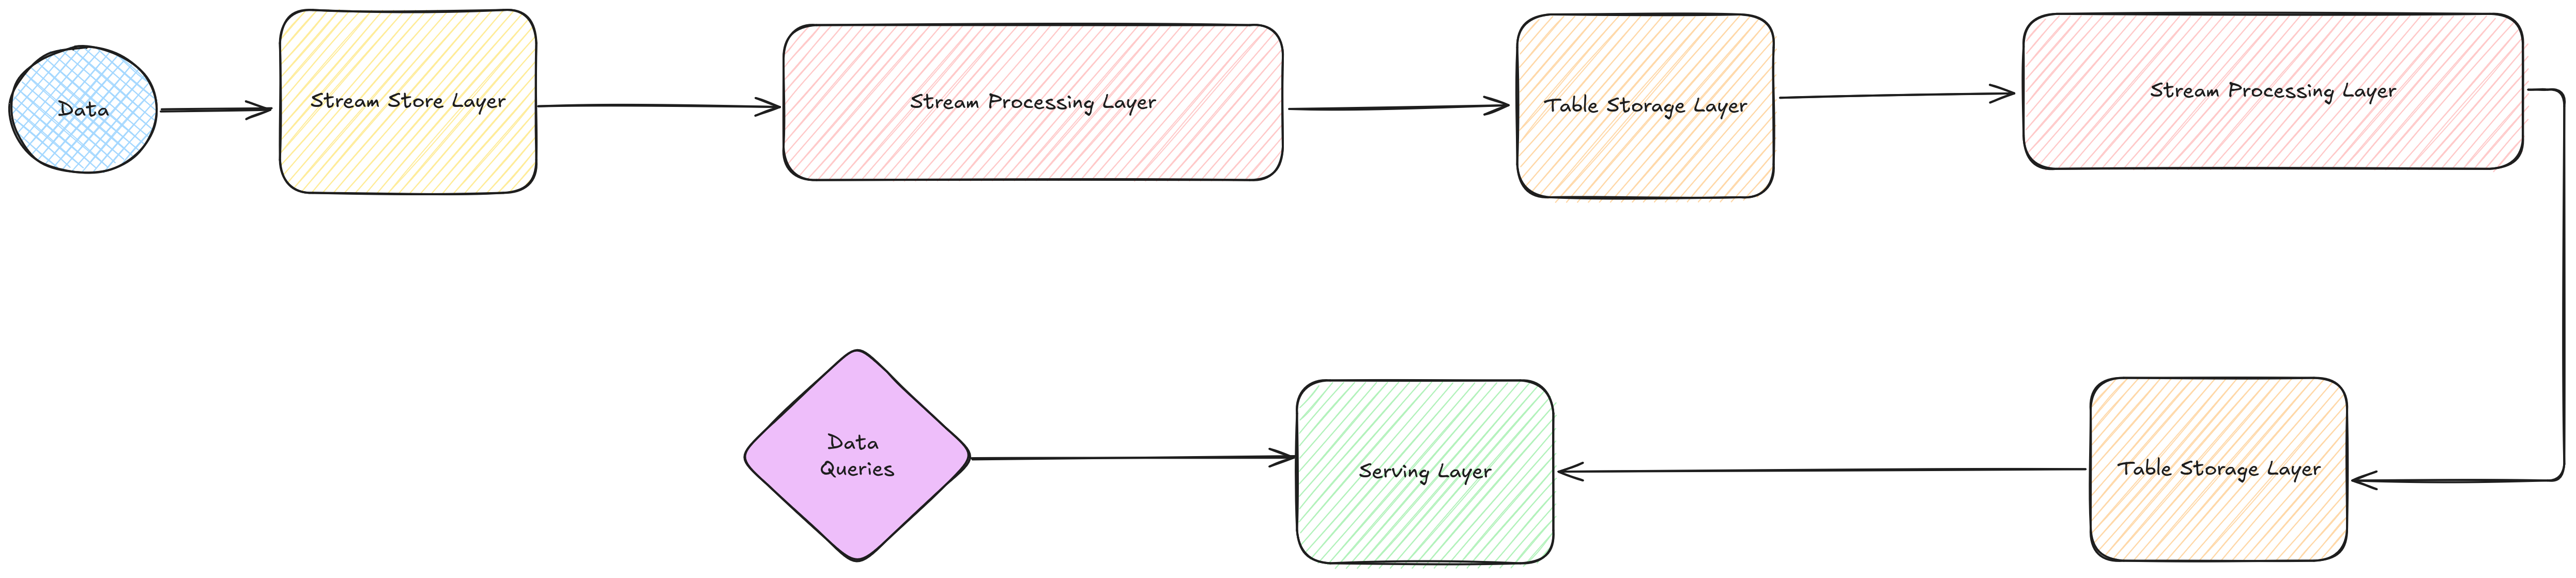
\includegraphics[width=0.8\textwidth]{teorico/delta.png}
\caption{Diagrama de la Arquitectura Delta}
\label{fig:arquitectura_delta}
\end{figure}

\subsection{Capacidades}
\begin{itemize}
    \item Garantiza características ACID para un sistema distribuido
    \item Reduce los costos de almacenamiento y procesamiento de la información 
    \item Define una fuente de verdad única que puede ser usada por todos los procesos de análisis
    \item Reduce la cantidad de código que se debe mantener
    \item Permite agregar nuevas fuentes de datos sin necesidad de cambios en los procesos de análisis
\end{itemize}

\subsection{Desafíos}
\begin{itemize}
    \item La latencia es un problema si se necesitan capacidades de análisis en tiempo real
    \item Se requieren compromisos de latencia y rendimiento por el problema de "Manejo de archivos pequeños"
    \item Si el Catalog Layer no se construye correctamente no es posible que la arquitectura escale
\end{itemize}